

\begin{center}
\thispagestyle{empty}
%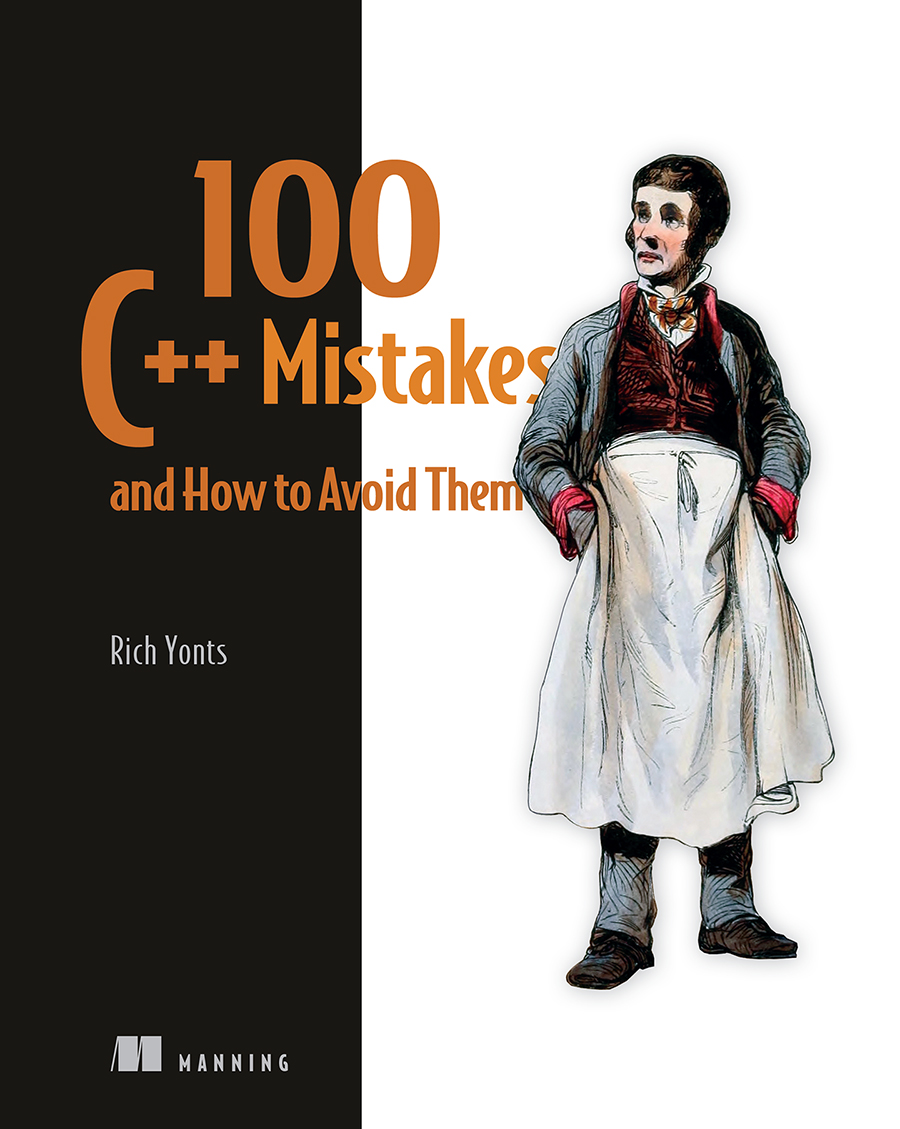
\includegraphics[width=\textwidth,height=\textheight,keepaspectratio]{cover.png}
\begin{tikzpicture}[remember picture, overlay, inner sep=0pt]
\node at (current page.center)
{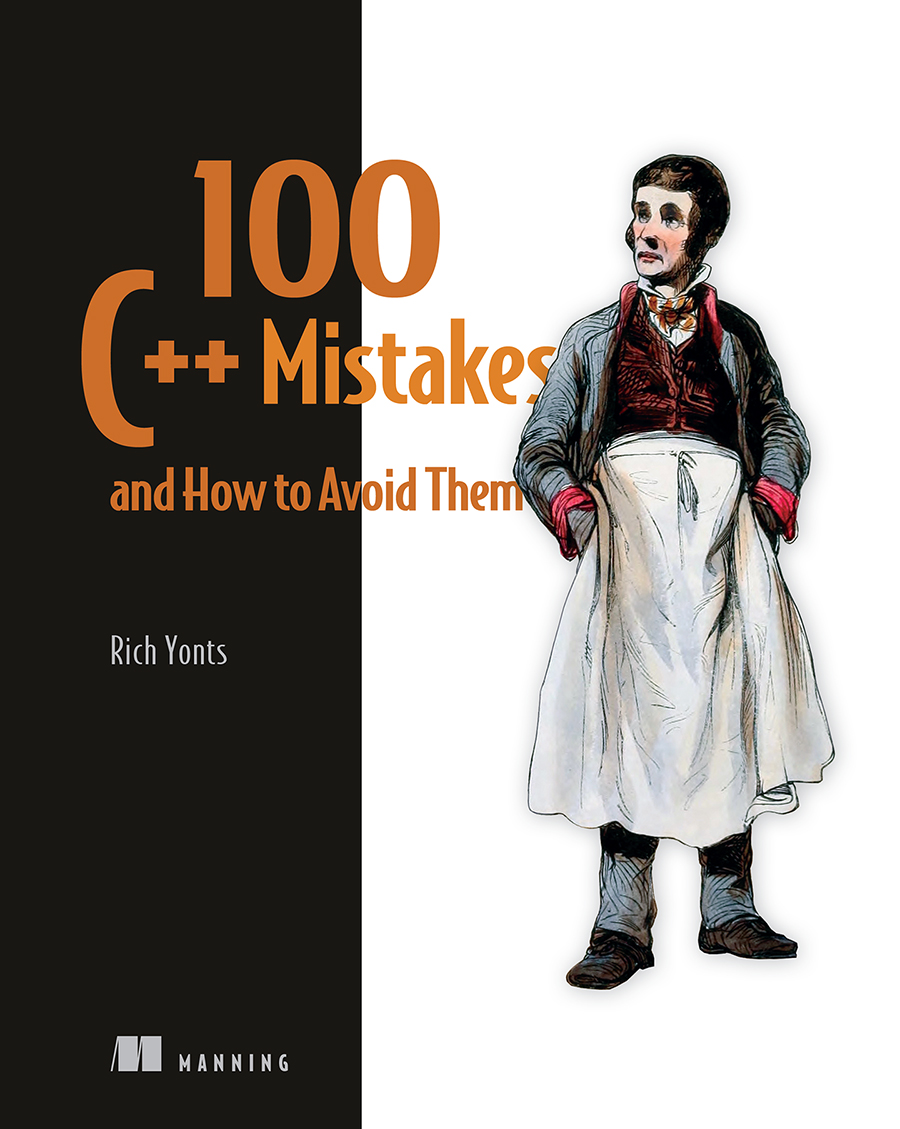
\includegraphics[width=\paperwidth, keepaspectratio=false]{cover.png}};
\end{tikzpicture}
\newpage
\thispagestyle{empty}
\huge
\textbf{C++编程避坑指南:100个常见错误及解决方案}
\\[9pt]
\normalsize
作者: Rich Yonts
\\[8pt]
\normalsize
译者:\href{https://github.com/xiaoweiChen/100-Cpp-Mistakes-and-How-to-Avoid-Them}{陈晓伟}
\\[8pt]
\end{center}

\newpage

\begin{comment}
\end{comment}

\myChapterNoContents{前言}{}{content/preface.tex}
\newpage

\myChapterNoContents{致谢}{}{content/acknowledgments.tex}
\newpage

\myChapterNoContents{关于本书}{}{content/about-this-book.tex}
\newpage

\myChapterNoContents{关于作者}{}{content/about-the-author.tex}
\newpage

\myChapterNoContents{封面插图}{}{content/about-the-cover-illustration.tex}
\newpage

\pagestyle{empty}
\tableofcontents
\newpage

\setsecnumdepth{section}

\myChapter{第1章}{C++:能力越大责任越大}{content/chapter1/0.tex}
\mySubsection{1.1.}{编程错误}{content/chapter1/1.tex}
\mySubsection{1.2.}{错误分析}{content/chapter1/2.tex}
\mySubsection{1.3.}{以错为师}{content/chapter1/3.tex}
\mySubsection{1.4.}{错迹可循}{content/chapter1/4.tex}
\mySubsection{1.5.}{本书结构}{content/chapter1/5.tex}
\mySubsection{1.6.}{总结}{content/chapter1/6.tex}
\newpage

\myPartGray{第一部分}{现代 C++}{content/part1/part.tex}
\newpage

\myChapter{第2章}{更好的现代C++:类和类型}{content/part1/chapter2/0.tex}
\mySubsection{2.1.}{错误 1: 未使用移动语义}{content/part1/chapter2/1.tex}
\mySubsection{2.2.}{错误 2: 使用空异常规范}{content/part1/chapter2/2.tex}
\mySubsection{2.3.}{错误 3: 未重写派生的虚函数}{content/part1/chapter2/3.tex}
\mySubsection{2.4.}{错误 4: 编写简单的或隐藏不需要的提供类成员}{content/part1/chapter2/4.tex}
\mySubsection{2.5.}{错误 5: 未使用类内初始化器}{content/part1/chapter2/5.tex}
\mySubsection{2.6.}{错误 6: 过度使用基于索引的循环}{content/part1/chapter2/6.tex}
\mySubsection{2.7.}{错误 7: 未使用nullptr}{content/part1/chapter2/7.tex}
\mySubsection{2.8.}{错误 8: 未使用unique\_ptr独占所有权}{content/part1/chapter2/8.tex}
\mySubsection{2.9.}{错误 9: 未使用shared\_ptr共享所有权}{content/part1/chapter2/9.tex}
\newpage

\myChapter{第3章}{更好的现代C++:通用编程}{content/part1/chapter3/0.tex}
\mySubsection{3.1.}{错误 10: 初始化时未使用if}{content/part1/chapter3/1.tex}
\mySubsection{3.2.}{错误 11: 未对变量使用类型推断}{content/part1/chapter3/2.tex}
\mySubsection{3.3.}{错误 12: 使用typedef}{content/part1/chapter3/3.tex}
\mySubsection{3.4.}{错误 13: 通用算法}{content/part1/chapter3/4.tex}
\mySubsection{3.5.}{错误 14: 未使用统一初始化}{content/part1/chapter3/5.tex}
\mySubsection{3.6.}{错误 15: 未使用就地初始化}{content/part1/chapter3/6.tex}
\mySubsection{3.7.}{错误 16: 未使用元组}{content/part1/chapter3/7.tex}
\mySubsection{3.8.}{错误 17: 未使用结构化绑定}{content/part1/chapter3/8.tex}
\newpage

\myChapter{第4章}{更好的现代C++:附加主题}{content/part1/chapter4/0.tex}
\mySubsection{4.1.}{错误 18: 未使用可变参数模板}{content/part1/chapter4/1.tex}
\mySubsection{4.2.}{错误 19: 使用全局命名空间枚举}{content/part1/chapter4/2.tex}
\mySubsection{4.3.}{错误 20: 未使用新的格式化功能}{content/part1/chapter4/3.tex}
\mySubsection{4.4.}{错误 21: 未使用容器的范围功能}{content/part1/chapter4/4.tex}
\mySubsection{4.5.}{错误 22: 编写非可移植的文件系统代码}{content/part1/chapter4/5.tex}
\mySubsection{4.6.}{错误 23: 编写过多的独立函数}{content/part1/chapter4/6.tex}
\mySubsection{4.7.}{错误 24: 手动定义笨拙的常量}{content/part1/chapter4/7.tex}
\mySubsection{4.8.}{错误 25: 编写模式匹配代码}{content/part1/chapter4/8.tex}
\newpage

\myPartGray{第二部分}{经典 C++}{content/part2/part.tex}
\newpage

\myChapter{第5章}{C语言的惯用法}{content/part2/chapter5/0.tex}
\mySubsection{5.1.}{错误 26: 总是在函数的顶部声明变量}{content/part2/chapter5/1.tex}
\mySubsection{5.2.}{错误 27: 宏依赖}{content/part2/chapter5/2.tex}
\mySubsection{5.3.}{错误 28: NULL的误解}{content/part2/chapter5/3.tex}
\mySubsection{5.4.}{错误 29: FILE访问文件}{content/part2/chapter5/4.tex}
\mySubsection{5.5.}{错误 30: 将整数值转为布尔值}{content/part2/chapter5/5.tex}
\mySubsection{5.6.}{错误 31: C风格的强制转换}{content/part2/chapter5/6.tex}
\mySubsection{5.7.}{错误 32: atoi转换文本}{content/part2/chapter5/7.tex}
\mySubsection{5.8.}{错误 33: C风格的字符串}{content/part2/chapter5/8.tex}
\mySubsection{5.9.}{错误 34: exit函数}{content/part2/chapter5/9.tex}
\mySubsection{5.10.}{错误 35: 优先选择数组}{content/part2/chapter5/10.tex}
\newpage

\myChapter{第6章}{更好的经典C++}{content/part2/chapter6/0.tex}
\mySubsection{6.1.}{错误 36: 使用 scanf 和 printf 进行输入和输出}{content/part2/chapter6/1.tex}
\mySubsection{6.2.}{错误 37: 过度使用 endl}{content/part2/chapter6/2.tex}
\mySubsection{6.3.}{错误 38: 使用 malloc 和 free 进行动态分配}{content/part2/chapter6/3.tex}
\mySubsection{6.4.}{错误 39: 使用联合(union)进行类型转换}{content/part2/chapter6/4.tex}
\mySubsection{6.5.}{错误 40: 使用 varargs 实现可变参数列表}{content/part2/chapter6/5.tex}
\mySubsection{6.6.}{错误 41: 类的初始化顺序}{content/part2/chapter6/6.tex}
\mySubsection{6.7.}{错误 42: 将非值类型添加到容器}{content/part2/chapter6/7.tex}
\mySubsection{6.8.}{错误 43: 首选索引}{content/part2/chapter6/8.tex}
\newpage

\myPartGray{第三部分}{前现代C++}{content/part3/part.tex}
\newpage

\myChapter{第7章}{创建类的不变量}{content/part3/chapter7/0.tex}
\mySubsection{7.1.}{类不变量确保类的正确设计}{content/part3/chapter7/1.tex}
\mySubsection{7.2.}{类设计中的错误}{content/part3/chapter7/2.tex}
\mySubsection{7.3.}{错误 44: 未能维护类不变量}{content/part3/chapter7/3.tex}
\mySubsection{7.4.}{错误 45: 未将类视为数据类型}{content/part3/chapter7/4.tex}
\mySubsection{7.5.}{错误 46: 未对方法建立基准}{content/part3/chapter7/5.tex}
\mySubsection{7.6.}{错误 47: 未能实现“三大”函数}{content/part3/chapter7/6.tex}
\mySubsection{7.7.}{错误 48: 仅为了代码复用而使用继承}{content/part3/chapter7/7.tex}
\mySubsection{7.8.}{错误 49: 过度使用默认构造函数}{content/part3/chapter7/8.tex}
\mySubsection{7.9.}{错误 50: 未能保持"is-a"关系}{content/part3/chapter7/9.tex}
\newpage

\myChapter{第8章}{保护类的不变量}{content/part3/chapter8/0.tex}
\mySubsection{8.1.}{保护类的不变量}{content/part3/chapter8/1.tex}
\mySubsection{8.2.}{错误 51: 编写非必要的访问器方法}{content/part3/chapter8/2.tex}
\mySubsection{8.3.}{错误 52: 提供脆弱的修改器}{content/part3/chapter8/3.tex}
\mySubsection{8.4.}{错误 53: 过度使用受保护的实例变量}{content/part3/chapter8/4.tex}
\mySubsection{8.5.}{错误 54: 混淆operator=和复制构造函数}{content/part3/chapter8/5.tex}
\mySubsection{8.6.}{错误 55: 误解浅复制与深复制}{content/part3/chapter8/6.tex}
\mySubsection{8.7.}{错误 56: 未调用基类的操作符}{content/part3/chapter8/7.tex}
\mySubsection{8.8.}{错误 57: 未在多态基类中使用虚析构函数}{content/part3/chapter8/8.tex}
\mySubsection{8.9.}{错误 58: 构造函数和析构函数中调用虚函数}{content/part3/chapter8/9.tex}
\mySubsection{8.10.}{错误 59: 尝试使用多态数组元素}{content/part3/chapter8/10.tex}
\mySubsection{8.11.}{错误 60: 未初始化所有实例变量}{content/part3/chapter8/11.tex}
\newpage

\myChapter{第9章}{类操作}{content/part3/chapter9/0.tex}
\mySubsection{9.1.}{错误 61: 对变量遮蔽的误解}{content/part3/chapter9/1.tex}
\mySubsection{9.2.}{错误 62: 允许复制唯一对象}{content/part3/chapter9/2.tex}
\mySubsection{9.3.}{错误 63: 未针对返回值优化进行编码}{content/part3/chapter9/3.tex}
\mySubsection{9.4.}{错误 64: 从复制赋值操作符不返回引用}{content/part3/chapter9/4.tex}
\mySubsection{9.5.}{错误 65: 忘记处理自我赋值}{content/part3/chapter9/5.tex}
\mySubsection{9.6.}{错误 66: 对前缀和后缀形式的误解}{content/part3/chapter9/6.tex}
\mySubsection{9.7.}{错误 67: 误导性的隐式转换操作符}{content/part3/chapter9/7.tex}
\mySubsection{9.8.}{错误 68: 过度使用隐式转换构造函数}{content/part3/chapter9/8.tex}
\mySubsection{9.9.}{错误 69: 过于关注独立操作符}{content/part3/chapter9/9.tex}
\mySubsection{9.10.}{错误 70: 未能将非变异方法标记为常量}{content/part3/chapter9/10.tex}
\mySubsection{9.11.}{错误 71: 未能正确地标记类方法为静态}{content/part3/chapter9/11.tex}
\mySubsection{9.12.}{错误 72: 错误的选择成员函数和非成员函数}{content/part3/chapter9/12.tex}
\mySubsection{9.13.}{错误 73: 从访问器方法中错误地返回字符串}{content/part3/chapter9/13.tex}
\newpage

\myChapter{第10章}{异常与资源管理}{content/part3/chapter10/0.tex}
\mySubsection{10.1.}{使用异常}{content/part3/chapter10/1.tex}
\mySubsection{10.2.}{错误 74: 构造函数中抛出异常}{content/part3/chapter10/2.tex}
\mySubsection{10.3.}{错误 75: 析构函数中抛出异常}{content/part3/chapter10/3.tex}
\mySubsection{10.4.}{错误 76: 使用异常时的资源泄漏}{content/part3/chapter10/4.tex}
\mySubsection{10.5.}{错误 77: 未使用RAII模式}{content/part3/chapter10/5.tex}
\mySubsection{10.6.}{错误 78: 使用指针管理资源}{content/part3/chapter10/6.tex}
\mySubsection{10.7.}{错误 79: 混合new和delete的不同形式}{content/part3/chapter10/7.tex}
\mySubsection{10.8.}{错误 80: 信任异常说明}{content/part3/chapter10/8.tex}
\mySubsection{10.9.}{错误 81: 未使用引用捕获异常}{content/part3/chapter10/9.tex}
\newpage

\myChapter{第11章}{函数与编码}{content/part3/chapter11/0.tex}
\mySubsection{11.1.}{设计考量}{content/part3/chapter11/1.tex}
\mySubsection{11.2.}{错误 82: 未使用默认参数}{content/part3/chapter11/2.tex}
\mySubsection{11.3.}{错误 83: 未能使用断言}{content/part3/chapter11/3.tex}
\mySubsection{11.4.}{错误 84: 返回局部对象的指针或引用}{content/part3/chapter11/4.tex}
\mySubsection{11.5.}{错误 85: 使用输出参数}{content/part3/chapter11/5.tex}
\mySubsection{11.6.}{错误 86: 参数类型的错误使用}{content/part3/chapter11/6.tex}
\mySubsection{11.7.}{错误 87: 依赖参数求值顺序}{content/part3/chapter11/7.tex}
\mySubsection{11.8.}{错误 88: 传递参数过多}{content/part3/chapter11/8.tex}
\mySubsection{11.9.}{错误 89: 函数过长且行为复杂}{content/part3/chapter11/9.tex}
\mySubsection{11.10.}{错误 90: 职能过多的函数}{content/part3/chapter11/10.tex}
\newpage

\myChapter{第12章}{通用编码}{content/part3/chapter12/0.tex}
\mySubsection{12.1.}{错误 91: 不正确处理除以零}{content/part3/chapter12/1.tex}
\mySubsection{12.2.}{错误 92: 不正确地使用循环中的continue}{content/part3/chapter12/2.tex}
\mySubsection{12.3.}{错误 93: 未能将已删除的指针设置为NULL}{content/part3/chapter12/3.tex}
\mySubsection{12.4.}{错误 94: 未能直接返回计算得到的布尔值}{content/part3/chapter12/4.tex}
\mySubsection{12.5.}{错误 95: 对表达式的利用不足}{content/part3/chapter12/5.tex}
\mySubsection{12.6.}{错误 96: 使用多余的else}{content/part3/chapter12/6.tex}
\mySubsection{12.7.}{错误 97: 未使用辅助函数}{content/part3/chapter12/7.tex}
\mySubsection{12.8.}{错误 98: 错误地比较浮点数值}{content/part3/chapter12/8.tex}
\mySubsection{12.9.}{错误 99: 浮点数到整数的赋值}{content/part3/chapter12/9.tex}
\mySubsection{12.10.}{错误 100: 忽略编译器警告}{content/part3/chapter12/10.tex}
\newpage

\begin{comment}
\end{comment}
